
\section{\trIsofibration{}的\trPullback}\label{sec:pullbacks-of-isofibrations}

\trInfinityCosmos{}中\trIsofibration{}之塔的\trPullback{}与\trLimit{}在%
\trHomotopyTwoCategory{}中也具有弱 2 维\trUniversalProperty，不过我们通常转而%
利用\trSimpliciallyEnrichedLimit{}的严格\trUniversalProperty。然而，%
\trPullback{}的弱 2 维\trUniversalProperty{}可用于证明：\trEquivalence{}沿%
\trIsofibration{}拉回后仍是\trEquivalence{}；而这又可用于确立%
\trInfinityCosmos{}中\trPullback{}的\trEquivalence{}不变性。

\begin{proposition}[\trPullback{}的弱\trUniversalProperty]\label{prop:pullback-weak-universal-property}
\trInfinityCosmos{}中沿一个\trFunctor{}的\trIsofibration{}之\trPullback%
\begin{center}
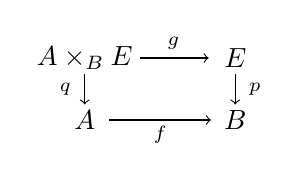
\begin{tikzpicture}[x=1.6em,y=1.6em]
  \node (tl) at (0,1.4) {$A\times_BE$};
  \node (tr) at (3.4,1.4) {$E$};
  \node (bl) at (0,0) {$A$};
  \node (br) at (3.4,0) {$B$};
  \draw[->] (1.25,1.4) -- (2.8,1.4);
  \node at (2.0,1.74) {$\scriptstyle g$};
  \draw[->] (0,1.05) -- (0,0.35);
  \node at (-0.44,0.7) {$\scriptstyle q$};
  \node at (0.48,0.78) {$\scriptstyle\lrcorner$};
  \draw[->] (3.4,1.05) -- (3.4,0.35);
  \node at (3.84,0.7) {$\scriptstyle p$};
  \draw[->] (0.55,0) -- (2.85,0);
  \node at (1.7,-0.34) {$\scriptstyle f$};
\end{tikzpicture}
\end{center}
在\trHomotopyTwoCategory{}中具有由下述三种运算给出的弱\trUniversalProperty{}：
\begin{enumerate}[label=(\roman*)]
\item \textbf{1-\trCell{}归纳：}在拉回图表所赖的\trCospan{}上方，满足%
$pe=f\alpha$ 的交换方块都唯一地穿过拉回方块分解
\begin{center}
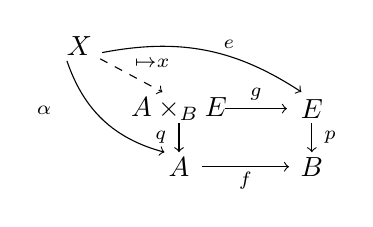
\begin{tikzpicture}[x=1.5em,y=1.5em]
  \node (X) at (0,2.9) {$X$};
  \node (tl) at (2.4,1.4) {$A\times_BE$};
  \node (tr) at (5.6,1.4) {$E$};
  \node (bl) at (2.4,0) {$A$};
  \node (br) at (5.6,0) {$B$};
  \draw[->,dashed] (0.5,2.6) -- (2.0,1.8);
  \node at (1.75,2.5) {$\scriptstyle\mapsto x$};
  \draw[->] (0.55,2.75) to[bend left=22] (5.35,1.8);
  \node at (3.6,2.95) {$\scriptstyle e$};
  \draw[->] (-0.3,2.55) to[bend right=28] (2.05,0.35);
  \node at (-0.85,1.35) {$\scriptstyle\alpha$};
  \draw[->] (3.5,1.4) -- (5.0,1.4);
  \node at (4.25,1.74) {$\scriptstyle g$};
  \draw[->] (2.4,1.05) -- (2.4,0.35);
  \node at (1.96,0.7) {$\scriptstyle q$};
  \node at (2.88,0.78) {$\scriptstyle\lrcorner$};
  \draw[->] (5.6,1.05) -- (5.6,0.35);
  \node at (6.04,0.7) {$\scriptstyle p$};
  \draw[->] (2.95,0) -- (5.05,0);
  \node at (4.0,-0.34) {$\scriptstyle f$};
\end{tikzpicture}
\end{center}
\item \textbf{2-\trCell{}归纳：}给定\trFunctor{} $x,x'\colon X\to A\times_BE$ 与%
\trNaturalTransformation{} $\alpha\colon qx\Rightarrow qx'$、%
$\epsilon\colon gx\Rightarrow gx'$，使得 $p\epsilon=f\alpha$，则存在%
\trNaturalTransformation{} $\tau\colon x\Rightarrow x'$，使得 $q\tau=\alpha$%
且 $g\tau=\epsilon$。
\item \textbf{2-\trCell{}保守性：}对任何
\begin{center}
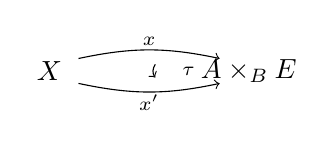
\begin{tikzpicture}[x=1.5em,y=1.5em]
  \node (X) at (0,0) {$X$};
  \node (M) at (4.8,0) {$A\times_BE$};
  \draw[->] (0.7,0.3) to[bend left=12] (4.1,0.3);
  \node at (2.4,0.72) {$\scriptstyle x$};
  \draw[->] (0.7,-0.3) to[bend right=12] (4.1,-0.3);
  \node at (2.4,-0.76) {$\scriptstyle x'$};
  \draw[->] (2.55,0.16) to[bend right=35] (2.55,-0.16);
  \node at (3.35,0.0) {$\scriptstyle\tau$};
\end{tikzpicture}
\end{center}
若 $q\tau$ 与 $g\tau$ 皆为\trIsomorphism{}，则 $\tau$ 是\trIsomorphism{}。
\end{enumerate}
\end{proposition}

\begin{proof}
对由\trQuasiCategory{}构成的如下\trPullback{}图表应用引理 3.1.5
\begin{center}
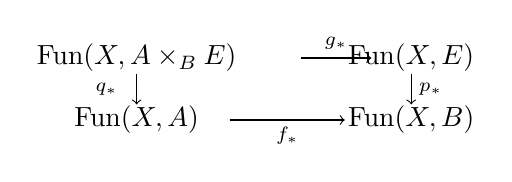
\begin{tikzpicture}[x=1.6em,y=1.6em]
  \node (tl) at (0,1.4) {$\mathrm{Fun}(X,A\times_BE)$};
  \node (tr) at (6.2,1.4) {$\mathrm{Fun}(X,E)$};
  \node (bl) at (0,0) {$\mathrm{Fun}(X,A)$};
  \node (br) at (6.2,0) {$\mathrm{Fun}(X,B)$};
  \draw[->] (3.7,1.4) -- (5.3,1.4);
  \node at (4.5,1.74) {$\scriptstyle g_{*}$};
  \draw[->] (0,1.05) -- (0,0.35);
  \node at (-0.68,0.7) {$\scriptstyle q_{*}$};
  \node at (0.48,0.78) {$\scriptstyle\lrcorner$};
  \draw[->] (6.2,1.05) -- (6.2,0.35);
  \node at (6.64,0.7) {$\scriptstyle p_{*}$};
  \draw[->] (2.1,0) -- (4.7,0);
  \node at (3.4,-0.36) {$\scriptstyle f_{*}$};
\end{tikzpicture}
\end{center}
即可观察到：\trHomCategory{}之间的自然映射
\[
\mathrm{hFun}(X,A\times_BE)\longrightarrow
\mathrm{hFun}(X,A)\times_{\mathrm{hFun}(X,B)}\mathrm{hFun}(X,E)
\]
是一个对象上双射的\trSmotheringFunctor{}。对象上的双射性由 1-\trCell{}归纳%
表达，满性由 2-\trCell{}归纳表达，而保守性由 2-\trCell{}保守性表达。
\end{proof}

\begin{digression}[\trWeaklyCartesianSquare]\label{dig:weakly-cartesian-squares}
平行\trIsofibration{}之间的一个交换方块是\textbf{\trWeaklyCartesian}%
（weakly cartesian），若其到\trPullback{}的诱导映射是一个\trEquivalence{}：
\begin{center}
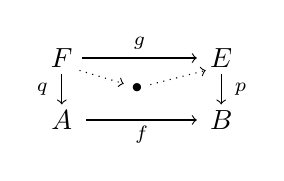
\begin{tikzpicture}[x=1.6em,y=1.6em]
  \node (tl) at (0,1.4) {$F$};
  \node (tr) at (3.6,1.4) {$E$};
  \node (bl) at (0,0) {$A$};
  \node (br) at (3.6,0) {$B$};
  \draw[->] (0.45,1.4) -- (3.05,1.4);
  \node at (1.75,1.74) {$\scriptstyle g$};
  \draw[->] (0,1.05) -- (0,0.35);
  \node at (-0.44,0.7) {$\scriptstyle q$};
  \draw[->] (3.6,1.05) -- (3.6,0.35);
  \node at (4.04,0.7) {$\scriptstyle p$};
  \draw[->] (0.55,0) -- (3.05,0);
  \node at (1.8,-0.34) {$\scriptstyle f$};
  \draw[->,dotted] (0.4,1.12) -- (1.4,0.82);
  \draw[->,dotted] (2.0,0.8) -- (3.25,1.12);
  \node at (1.7,0.72) {$\scriptstyle\bullet$};
  \node at (2.25,0.5) {$\scriptstyle\lrcorner$};
\end{tikzpicture}
\end{center}
\trWeaklyCartesianSquare{}同样满足 2-\trCell{}归纳与 2-\trCell{}保守性，还%
满足一种经过修改的 1-\trCell{}归纳性质：此时本质唯一的诱导\trFunctor{}在%
$B$ 上严格交换，而在 $E$ 上至多相差一个同构——该同构沿 $p$ 投影为恒同——%
[110, 3.5.4]。
\end{digression}

由\trPullback{}的\trBicategory\trUniversalProperty{}可以推出：\trInfinityCosmos{}%
都是\textbf{\trRightProper}（right proper）——意即任何\trEquivalence{}沿%
\trIsofibration{}的\trPullback{}都定义出一个\trEquivalence{}。

\begin{proposition}\label{prop:pullback-equivalence}
在任何\trInfinityCosmos{}中，\trEquivalence{}沿\trIsofibration{}的%
\trPullback{}是一个\trEquivalence{}。
\begin{center}
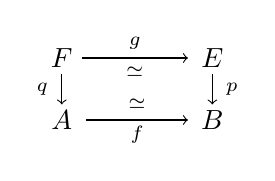
\begin{tikzpicture}[x=1.6em,y=1.6em]
  \node (tl) at (0,1.4) {$F$};
  \node (tr) at (3.4,1.4) {$E$};
  \node (bl) at (0,0) {$A$};
  \node (br) at (3.4,0) {$B$};
  \draw[->] (0.45,1.4) -- (2.85,1.4);
  \node at (1.65,1.74) {$\scriptstyle g$};
  \node at (1.65,1.08) {$\scriptstyle\simeq$};
  \draw[->] (0,1.05) -- (0,0.35);
  \node at (-0.44,0.7) {$\scriptstyle q$};
  \node at (0.48,0.78) {$\scriptstyle\lrcorner$};
  \draw[->] (3.4,1.05) -- (3.4,0.35);
  \node at (3.84,0.7) {$\scriptstyle p$};
  \draw[->] (0.55,0) -- (2.85,0);
  \node at (1.7,-0.34) {$\scriptstyle f$};
  \node at (1.7,0.36) {$\scriptstyle\simeq$};
\end{tikzpicture}
\end{center}
\end{proposition}

\begin{proof}
由命题 2.1.12，我们可以选取 $f$ 的一个\trAdjointEquivalence{}逆 $f^{-1}$，并%
挑选可逆 2-\trCell{} $\alpha\colon\mathrm{id}_A\cong f^{-1}f$ 与%
$\beta\colon ff^{-1}\cong\mathrm{id}_B$，使之在\trHomotopyTwoCategory{}中%
满足\trTriangleEqualities{}。\footnote{正是因为这一点，我们使用的才是拉回的%
\trBicategory\trUniversalProperty，而非单纯富集的\trUniversalProperty。}
既然映射 $p$ 是\trIsofibration{}，我们便可利用命题 1.4.9 把同构%
$\beta p\colon ff^{-1}p\cong p$ 沿 $p$ 提升，以定义一个\trIsomorphism{}%
$\epsilon\colon e\cong\mathrm{id}_E$，其余定义域为 $\mathrm{id}_E\colon E\to E$。%
由构造有 $pe=ff^{-1}p$，故由 1-\trCell{}归纳，对 $(f^{-1}p,e)$ 便诱导出映射%
$g^{-1}\colon E\to F$，使得 $qg^{-1}=f^{-1}p$ 且 $gg^{-1}=e$。这样我们便%
得到一个\trIsomorphism{} $\epsilon\colon gg^{-1}\cong\mathrm{id}_E$，满足%
$p\epsilon=\beta p$。

现在，据\cref{prop:pullback-weak-universal-property}的 2-\trCell{}归纳与%
保守性，为定义一个\trIsomorphism{} $\mathrm{id}_F\cong g^{-1}g$，只需给出%
如下一对\trIsomorphism
\[
\alpha q\colon q\cong f^{-1}fq=f^{-1}pg=qg^{-1}g
\qquad\text{以及}\qquad
\epsilon^{-1}g\colon g\cong gg^{-1}g
\]
使得 $f\alpha q=p\epsilon^{-1}g$。后一等式之所以成立，是因为对%
\trAdjointEquivalence{} $f\dashv f^{-1}$ 而言，据三角等式%
$\beta f\cdot f\alpha=\mathrm{id}_f$，有%
$p\epsilon^{-1}g=\beta^{-1}pg=\beta^{-1}fq=f\alpha q$。于是，我们可以把 $f$ %
的逆\trEquivalence{}数据加以提升，以定义其\trPullback{} $g$ 的%
逆\trEquivalence{}。
\end{proof}

作为\trRightProperness{}的推论，在任何\trInfinityCosmos{}中，\trPullback{}%
都是一个\trEquivalence{}不变的构造。

\begin{proposition}\label{prop:pullback-invariance}
给定任意\trInfinityCosmos{}中一个由\trIsofibration{}与\trEquivalence{}构成%
的\trDiagram
\begin{center}
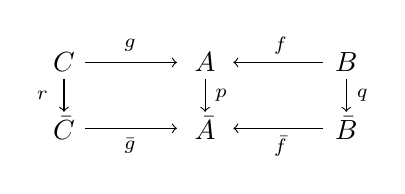
\begin{tikzpicture}[x=1.7em,y=1.7em]
  \node (tl) at (0,1.4) {$C$};
  \node (tm) at (3.0,1.4) {$A$};
  \node (tr) at (6.0,1.4) {$B$};
  \node (bl) at (0,0) {$\bar{C}$};
  \node (bm) at (3.0,0) {$\bar{A}$};
  \node (brr) at (6.0,0) {$\bar{B}$};
  \draw[->] (0.45,1.4) -- (2.4,1.4);
  \node at (1.4,1.76) {$\scriptstyle g$};
  \draw[->] (5.5,1.4) -- (3.6,1.4);
  \node at (4.6,1.76) {$\scriptstyle f$};
  \draw[->] (0.45,0) -- (2.4,0);
  \node at (1.4,-0.38) {$\scriptstyle\bar{g}$};
  \draw[->] (5.5,0) -- (3.6,0);
  \node at (4.6,-0.38) {$\scriptstyle\bar{f}$};
  \draw[->] (0,1.05) -- (0,0.35);
  \node at (-0.46,0.7) {$\scriptstyle r$};
  \draw[->] (3.0,1.05) -- (3.0,0.35);
  \node at (3.34,0.7) {$\scriptstyle p$};
  \draw[->] (6.0,1.05) -- (6.0,0.35);
  \node at (6.34,0.7) {$\scriptstyle q$};
\end{tikzpicture}
\end{center}
上下两行各自的\trPullback{}之间的诱导映射%
$C\times_AB\to\bar{C}\times_{\bar{A}}\bar{B}$ 仍是\trEquivalence{}。
\end{proposition}

\begin{proof}
利用引理 1.2.19 作因子分解，我们可以把映射 $\bar{g}$ 替换成一个%
\trIsofibration{}。据\trTwoOfThreeProperty{}与%
\cref{prop:pullback-equivalence}的\trRightProperness，该\trIsofibration{}沿%
\trEquivalence{} $p$ 的\trPullback{}便\trEquivalence{}于映射 $g$：
\begin{center}
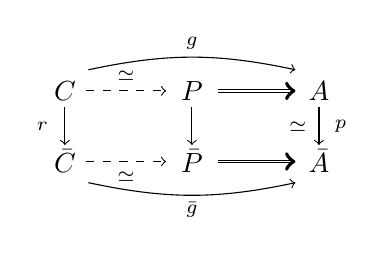
\begin{tikzpicture}[x=1.7em,y=1.7em]
  \node (C) at (0,1.4) {$C$};
  \node (P) at (2.7,1.4) {$P$};
  \node (A) at (5.4,1.4) {$A$};
  \node (Cb) at (0,-0.1) {$\bar{C}$};
  \node (Pb) at (2.7,-0.1) {$\bar{P}$};
  \node (Ab) at (5.4,-0.1) {$\bar{A}$};
  \draw[->] (0.5,1.85) to[bend left=12] (4.9,1.85);
  \node at (2.7,2.42) {$\scriptstyle g$};
  \draw[->] (0.5,-0.55) to[bend right=12] (4.9,-0.55);
  \node at (2.7,-1.12) {$\scriptstyle\bar{g}$};
  \draw[->,dashed] (0.45,1.4) -- (2.15,1.4);
  \node at (1.3,1.72) {$\scriptstyle\simeq$};
  \draw[double,->] (3.25,1.4) -- (4.9,1.4);
  \draw[->,dashed] (0.45,-0.1) -- (2.15,-0.1);
  \node at (1.3,-0.42) {$\scriptstyle\simeq$};
  \draw[double,->] (3.25,-0.1) -- (4.9,-0.1);
  \draw[->] (0,1.05) -- (0,0.25);
  \node at (-0.48,0.65) {$\scriptstyle r$};
  \draw[->] (2.7,1.05) -- (2.7,0.25);
  \draw[->] (5.4,1.05) -- (5.4,0.25);
  \node at (5.86,0.65) {$\scriptstyle p$};
  \node at (4.95,0.65) {$\scriptstyle\simeq$};
  \node at (3.2,1.02) {$\scriptstyle\lrcorner$};
\end{tikzpicture}
\end{center}
\begin{center}
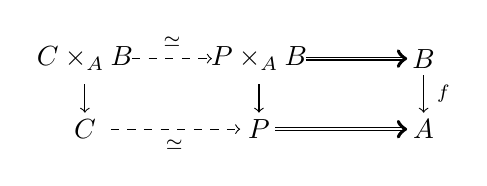
\begin{tikzpicture}[x=1.7em,y=1.7em]
  \node (Cg) at (0,1.4) {$C\times_AB$};
  \node (Pg) at (3.7,1.4) {$P\times_AB$};
  \node (B)  at (7.2,1.4) {$B$};
  \node (C)  at (0,-0.1) {$C$};
  \node (P)  at (3.7,-0.1) {$P$};
  \node (A)  at (7.2,-0.1) {$A$};
  \draw[->,dashed] (1.0,1.4) -- (2.7,1.4);
  \node at (1.85,1.76) {$\scriptstyle\simeq$};
  \draw[double,->] (4.7,1.4) -- (6.85,1.4);
  \draw[->,dashed] (0.55,-0.1) -- (3.3,-0.1);
  \node at (1.9,-0.42) {$\scriptstyle\simeq$};
  \draw[double,->] (4.05,-0.1) -- (6.85,-0.1);
  \draw[->] (0,0.85) -- (0,0.25);
  \draw[->] (3.7,0.85) -- (3.7,0.25);
  \draw[->] (7.2,1.05) -- (7.2,0.25);
  \node at (7.62,0.65) {$\scriptstyle f$};
  \node at (0.9,0.8) {$\scriptstyle\lrcorner$};
  \node at (4.6,0.8) {$\scriptstyle\lrcorner$};
\end{tikzpicture}
\end{center}

再由\trRightProperness，$P\twoheadrightarrow A$ 沿 $f$ 的\trPullback{}与%
$g\colon C\to A$ 沿 $f$ 的\trPullback{}\trEquivalence{}，对下方水平映射%
亦然。于是不失一般性，我们可以假设题设中的映射 $g$ 与 $\bar{g}$ 都是%
\trIsofibration{}，而且左手方块是一个\trPullback{}。

在这些新假设之下，立方体的顶面、底面与正面都是拉回方块：
\begin{center}
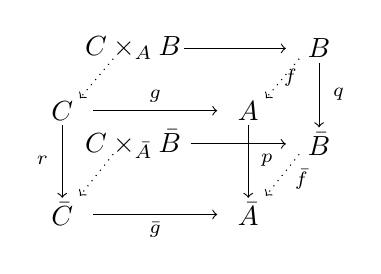
\begin{tikzpicture}[x=1.6em,y=1.5em]
  \node (Btl) at (1.6,4.0) {$C\times_AB$};
  \node (Btr) at (5.8,4.0) {$B$};
  \node (Bbl) at (1.6,1.7) {$C\times_{\bar{A}}\bar{B}$};
  \node (Bbr) at (5.8,1.7) {$\bar{B}$};
  \node (Ftl) at (0,2.5) {$C$};
  \node (Ftr) at (4.2,2.5) {$A$};
  \node (Fbl) at (0,0) {$\bar{C}$};
  \node (Fbr) at (4.2,0) {$\bar{A}$};
  \draw[->] (0.7,2.5) -- (3.5,2.5);
  \node at (2.1,2.85) {$\scriptstyle g$};
  \draw[->] (0.7,0) -- (3.5,0);
  \node at (2.1,-0.36) {$\scriptstyle\bar{g}$};
  \draw[->] (0,2.15) -- (0,0.4);
  \node at (-0.45,1.3) {$\scriptstyle r$};
  \draw[->] (4.2,2.15) -- (4.2,0.4);
  \node at (4.62,1.3) {$\scriptstyle p$};
  \draw[->] (2.75,4.0) -- (5.05,4.0);
  \draw[->] (2.9,1.7) -- (5.05,1.7);
  \draw[->] (5.8,3.65) -- (5.8,2.1);
  \node at (6.24,2.9) {$\scriptstyle q$};
  \draw[->,dotted] (1.15,3.75) -- (0.4,2.8);
  \draw[->,dotted] (5.35,3.75) -- (4.6,2.8);
  \node at (5.15,3.3) {$\scriptstyle f$};
  \draw[->,dotted] (1.15,1.45) -- (0.4,0.45);
  \draw[->,dotted] (5.35,1.45) -- (4.6,0.45);
  \node at (5.4,0.85) {$\scriptstyle\bar{f}$};
  \node at (2.2,3.62) {$\scriptstyle\lrcorner$};
  \node at (0.48,2.12) {$\scriptstyle\lrcorner$};
  \node at (2.2,1.32) {$\scriptstyle\lrcorner$};
\end{tikzpicture}
\end{center}
故由拉回的复合与消去，背面也是一个拉回方块。此时，诱导映射%
$C\times_AB\to\bar{C}\times_{\bar{A}}\bar{B}$ 是等价 $q$ 沿一个%
\trIsofibration{}的\trPullback{}，从而据\cref{prop:pullback-equivalence}是%
\trEquivalence{}。
\end{proof}

\subsection*{练习}

\begin{exercise}\label{ex:pullback-isomorphic-functors}
利用\cref{prop:pullback-weak-universal-property}证明：对任何%
\trIsofibration{}以及一对平行的、相互\trIsomorphism{}的\trFunctor
\begin{center}
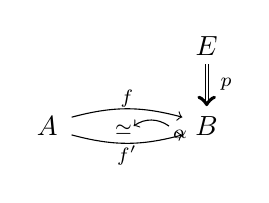
\begin{tikzpicture}[x=1.6em,y=1.6em]
  \node (A) at (0,0) {$A$};
  \node (B) at (3.6,0) {$B$};
  \node (E) at (3.6,1.8) {$E$};
  \draw[double,->] (3.6,1.4) -- (3.6,0.45);
  \node at (4.04,0.95) {$\scriptstyle p$};
  \draw[->] (0.55,0.2) to[bend left=15] (3.05,0.2);
  \node at (1.8,0.62) {$\scriptstyle f$};
  \draw[->] (0.55,-0.2) to[bend right=15] (3.05,-0.2);
  \node at (1.8,-0.66) {$\scriptstyle f'$};
  \draw[->] (2.75,0.0) to[bend right=35] (1.95,0.0);
  \node at (3.0,-0.18) {$\scriptstyle\alpha$};
  \node at (1.72,-0.08) {$\scriptstyle\simeq$};
\end{tikzpicture}
\end{center}
它们的\trPullback{}在 $A$ 上\trEquivalence{}。
\end{exercise}

\begin{exercise}\label{ex:towers-weak-universal-property}
陈述并证明一个与\cref{prop:pullback-weak-universal-property}相类似的结果，刻画%
\trIsofibration{}之塔的\trLimit{}的\trBicategory\trUniversalProperty。
\end{exercise}

\begin{exercise}\label{ex:towers-limits-equivalence}
利用\cref{ex:towers-weak-universal-property}的结果证明：\trIsofibration{}之塔之间的%
一个自然\trEquivalence{}——通过改编\cref{prop:pullback-equivalence}与%
\cref{prop:pullback-invariance}的证明中所给出的构造——诱导出它们的\trLimit{}之间的%
一个\trEquivalence。
\end{exercise}
